\documentclass[11pt,a4paper]{article}
\usepackage[T1]{fontenc}
\usepackage[utf8]{inputenc}
\usepackage{lmodern}
\usepackage[margin=22mm,headheight=16pt]{geometry}
\usepackage{amsmath,amssymb,graphicx,array,longtable,booktabs}
\usepackage{microtype,xcolor,hyperref,xurl,fancyhdr}
\definecolor{Navy}{HTML}{17324D}
\definecolor{Teal}{HTML}{087F8C}
\definecolor{Gold}{HTML}{B88128}
\hypersetup{colorlinks=true,linkcolor=Navy,urlcolor=Teal,bookmarksnumbered=true,hypertexnames=false}
\setlength{\parindent}{0pt}
\setlength{\parskip}{6pt}
\setlength{\emergencystretch}{4em}
\setcounter{tocdepth}{1}
\pagestyle{fancy}\fancyhf{}
\fancyfoot[R]{\small\thepage}
\fancyfoot[L]{\small\sffamily Sharif University of Technology}
\renewcommand{\headrulewidth}{0.3pt}
\makeatletter
\renewcommand\section{\@startsection{section}{1}{\z@}{-3.2ex plus -1ex minus -.2ex}{1.6ex plus .2ex}{\normalfont\Large\sffamily\bfseries\color{Navy}}}
\renewcommand\subsection{\@startsection{subsection}{2}{\z@}{-2.5ex plus -1ex minus -.2ex}{1.2ex plus .2ex}{\normalfont\large\sffamily\bfseries\color{Teal}}}
\makeatother
\fancyhead[L]{\small\sffamily\color{Navy}Sharif University of Technology}\fancyhead[R]{\small\sffamily\color{Teal}Project Assignment}\begin{document}
\begin{titlepage}\centering\vspace*{7mm}

\includegraphics[width=31mm]{assets/sharif_emblem_en.png}\par\vspace{5mm}
{\Large\sffamily\bfseries\color{Navy}SHARIF UNIVERSITY OF TECHNOLOGY\par}
\vspace{2mm}{\sffamily Department of Electrical Engineering\par}
\vspace{17mm}{\color{Teal}\rule{\linewidth}{1.4pt}}\par\vspace{6mm}
{\large\sffamily\color{Teal}PROJECT ASSIGNMENT\par}
\vspace{8mm}{\huge\sffamily\bfseries\color{Navy}Seven-Bus Power-Flow and Contingency Analysis in PowerWorld\par}
\vspace{9mm}{\color{Gold}\rule{45mm}{1pt}}\par\vfill
\begin{minipage}{.88\linewidth}
{\sffamily\color{Teal}INSTRUCTOR / INSTRUCTORS}\par
Instructor not stated in supplied assignment\par\vspace{7mm}
{\sffamily\color{Teal}ACADEMIC CONTEXT}\par
Energy Systems Analysis\par\end{minipage}\vfill
\end{titlepage}
\tableofcontents\clearpage
\section{Purpose and modeling assumptions}

Solve unknown bus voltages and network complex-power flows for known loads, generation schedules, and operating limits. Use a balanced three-phase steady-state model represented by a one-line diagram. Power flow supports operational planning and contingency screening;\allowbreak{} a converged steady-state solution alone does not establish transient or small-signal stability. Choose base apparent power S\_\allowbreak{}base and voltage bases consistent with transformer ratios. In per unit, a quantity equals its actual value divided by its base. For three-phase bases, I\_\allowbreak{}base =\allowbreak{} S\_\allowbreak{}base/\allowbreak{}(sqrt(3)*V\_\allowbreak{}LL,base) and Z\_\allowbreak{}base =\allowbreak{} V\_\allowbreak{}LL,base\textasciicircum{}2/\allowbreak{}S\_\allowbreak{}base. Correctly convert equipment impedance to the chosen common base. The experiment uses S\_\allowbreak{}base =\allowbreak{} 100 MVA.

\begin{figure}[!htbp]\centering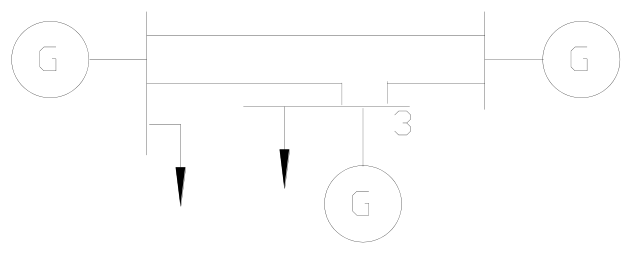
\includegraphics[width=\linewidth,height=.72\textheight,keepaspectratio]{assets/energy_assignment_p002_vector3.png}\caption{Diagram or recorded result: Purpose and modeling assumptions.}\label{fig:energy_assignment_p002_vector30}\end{figure}
\clearpage
\section{Nodal equations and bus types}

Let I =\allowbreak{} Y\_\allowbreak{}bus V and S\_\allowbreak{}i =\allowbreak{} P\_\allowbreak{}i+\allowbreak{}jQ\_\allowbreak{}i =\allowbreak{} V\_\allowbreak{}i*conj(I\_\allowbreak{}i). Net injection equals generation minus load. With Y\_\allowbreak{}ij =\allowbreak{} G\_\allowbreak{}ij+\allowbreak{}jB\_\allowbreak{}ij and angle difference theta\_\allowbreak{}i-theta\_\allowbreak{}j, P\_\allowbreak{}i =\allowbreak{} sum\_\allowbreak{}j abs(V\_\allowbreak{}i)*abs(V\_\allowbreak{}j)*(G\_\allowbreak{}ij*cos(theta\_\allowbreak{}i-theta\_\allowbreak{}j)+\allowbreak{}B\_\allowbreak{}ij*sin(theta\_\allowbreak{}i-theta\_\allowbreak{}j));\allowbreak{} Q\_\allowbreak{}i =\allowbreak{} sum\_\allowbreak{}j abs(V\_\allowbreak{}i)*abs(V\_\allowbreak{}j)*(G\_\allowbreak{}ij*sin(theta\_\allowbreak{}i-theta\_\allowbreak{}j)-B\_\allowbreak{}ij*cos(theta\_\allowbreak{}i-theta\_\allowbreak{}j)).


\begingroup\small\setlength{\tabcolsep}{3pt}\renewcommand{\arraystretch}{1.2}
\begin{longtable}{@{}p{0.3100\linewidth}p{0.3100\linewidth}p{0.3100\linewidth}@{}}
\toprule
\textbf{Bus type} & \textbf{Specified} & \textbf{Solved} \\ \midrule
\endfirsthead
\textbf{Bus type} & \textbf{Specified} & \textbf{Solved} \\ \midrule \endhead
Slack/\allowbreak{}swing & voltage magnitude and reference angle & real/\allowbreak{}reactive injection \\
PV/\allowbreak{}generator & real injection and voltage magnitude & angle and reactive injection \\
PQ/\allowbreak{}load & real and reactive injection & voltage magnitude and angle \\
\bottomrule\end{longtable}\endgroup

A slack bus balances losses and mismatch within the modeled connected network. Reactive-generation limits can cause a PV bus to become a PQ bus at its bound. Voltage limits and line/\allowbreak{}transformer ratings are additional operating constraints, not automatically satisfied by solving the equations.

\begingroup\small\setlength{\tabcolsep}{3pt}\renewcommand{\arraystretch}{1.18}\begin{longtable}{@{}p{0.1720\linewidth}p{0.1720\linewidth}p{0.1720\linewidth}p{0.1720\linewidth}p{0.1720\linewidth}@{}}
\caption{Nodal equations and bus types - numerical data and parameters.}\label{tab:energy_assignment_p003_table10}\\\toprule
\textbf{Bus type} & \textbf{P} & \textbf{Q} & \textbf{V} & \textbf{Angle (rad)} \\ \midrule\endfirsthead \textbf{Bus type} & \textbf{P} & \textbf{Q} & \textbf{V} & \textbf{Angle (rad)} \\ \midrule\endhead
Swing bus & Unknown & Unknown & Known & Known \\
Load bus & Known & Known & Unknown & Unknown \\
Generator bus & Known & Unknown & Known & Unknown \\
\bottomrule\end{longtable}\endgroup
\clearpage
\section{Gauss-Seidel method}

For A x =\allowbreak{} b, update x\_\allowbreak{}i using newly updated components before i and previous-iteration components after i. In power flow, replace unknown current injections by conj(S\_\allowbreak{}i/\allowbreak{}V\_\allowbreak{}i) to obtain the voltage iteration. For PQ buses use specified P/\allowbreak{}Q. At a PV bus compute reactive injection, check generation bounds, update angle, and enforce specified magnitude if the reactive control is feasible. The slack voltage remains fixed. State initialization, iteration order, tolerance, and maximum iterations. Nonconvergence can reflect initialization, conditioning, control limits, or an infeasible case. It does not by itself prove physical dynamic instability.

\section{Newton-Raphson method}

Linearize the nonlinear residual around the current state. The scalar method uses x\_\allowbreak{}next =\allowbreak{} x-f(x)/\allowbreak{}f'(x), a tangent step, rather than the distinct derivative-free secant method. For a vector system solve J*delta\_\allowbreak{}x =\allowbreak{} mismatch and update angles and PQ magnitudes with consistent signs. With n buses and m PQ buses, excluding the slack gives n-1+\allowbreak{}m unknowns and equations under the stated ordering. Check residual and step tolerances, reactive limits, and failed/\allowbreak{}singular solves. Newton often converges in fewer iterations than Gauss-Seidel, especially for large cases, but iterations and convergence are not universally independent of network size or operating condition. Each iteration requires Jacobian construction/\allowbreak{}factorization and additional storage.

\begin{figure}[!htbp]\centering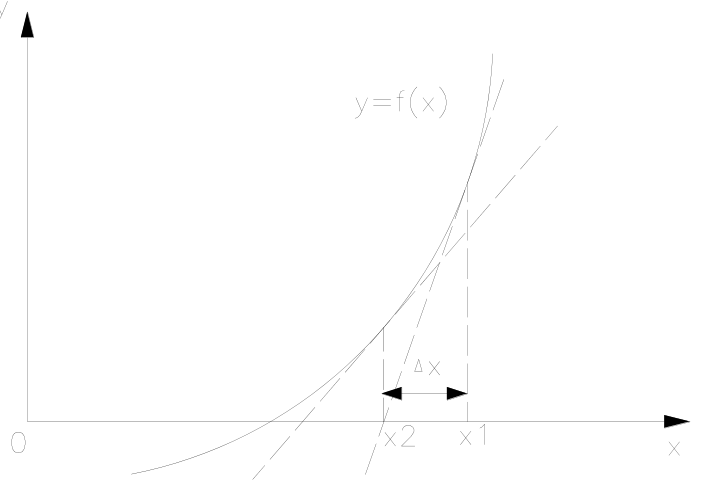
\includegraphics[width=\linewidth,height=.72\textheight,keepaspectratio]{assets/energy_assignment_p006_vector2.png}\caption{Diagram or recorded result: Newton-Raphson method.}\label{fig:energy_assignment_p006_vector20}\end{figure}
\clearpage
\section{Contingencies and PowerWorld workflow}

An N-1 screening removes one specified element and checks whether the remaining steady-state case satisfies operating criteria. The wider software also offers economic dispatch, OPF, and fault analysis. These available tools are background, not all required completed experiments. The examples illustrate a three-bus network, a Newton tangent step, a two-bus case, an OPF dialog, and a fault-analysis dialog.

\section{Seven-bus case data}

Use two generators and four loads with shunt capacitor banks at buses 3 and 7. The 345-kV lines have impedance 0.1019+\allowbreak{}j0.5912 ohm/\allowbreak{}km. Line lengths L1-L5 are 500,100,300,200,100 km. Transformers have reactance j0.1580 per unit. Generator maximum outputs are 100 MW. Line ratings are 100 MVA and transformer ratings 150 MVA. Participation factors are four at bus 1 and six at bus 2;\allowbreak{} unspecified parameters use the supplied defaults.


\begingroup\small\setlength{\tabcolsep}{3pt}\renewcommand{\arraystretch}{1.2}
\begin{longtable}{@{}p{0.0867\linewidth}p{0.0867\linewidth}p{0.0867\linewidth}p{0.0867\linewidth}p{0.0867\linewidth}p{0.0867\linewidth}p{0.0867\linewidth}p{0.0867\linewidth}p{0.0867\linewidth}@{}}
\toprule
\textbf{Bus} & \textbf{Pg MW} & \textbf{Qg/\allowbreak{}table MVAr} & \textbf{Pl MW} & \textbf{Ql MVAr} & \textbf{Type code} & \textbf{Qmax MVAr} & \textbf{Qmin MVAr} & \textbf{kV} \\ \midrule
\endfirsthead
\textbf{Bus} & \textbf{Pg MW} & \textbf{Qg/\allowbreak{}table MVAr} & \textbf{Pl MW} & \textbf{Ql MVAr} & \textbf{Type code} & \textbf{Qmax MVAr} & \textbf{Qmin MVAr} & \textbf{kV} \\ \midrule \endhead
1 & 55 & 32 & 0 & 0 & 2 & 40 & -6 & 34.5 \\
2 & 82 & 33 & 26 & 0 & 1 & 40 & -6 & 34.5 \\
3 & 0 & 37 & 50 & 34 & 3 & 0 & 0 & 345 \\
4 & 0 & 0 & 0 & 0 & 3 & 0 & 0 & 345 \\
5 & 0 & 0 & 0 & 0 & 3 & 0 & 0 & 345 \\
6 & 0 & 0 & 40 & 23 & 3 & 0 & 0 & 345 \\
7 & 0 & 10 & 20 & 15 & 3 & 0 & 0 & 345 \\
\bottomrule\end{longtable}\endgroup

Codes are 1 slack, 2 PV, 3 PQ. Reactive entries at buses 3/\allowbreak{}7 relate to the stated shunts and must not be mistaken for unrestricted generator controls.

\begin{figure}[!htbp]\centering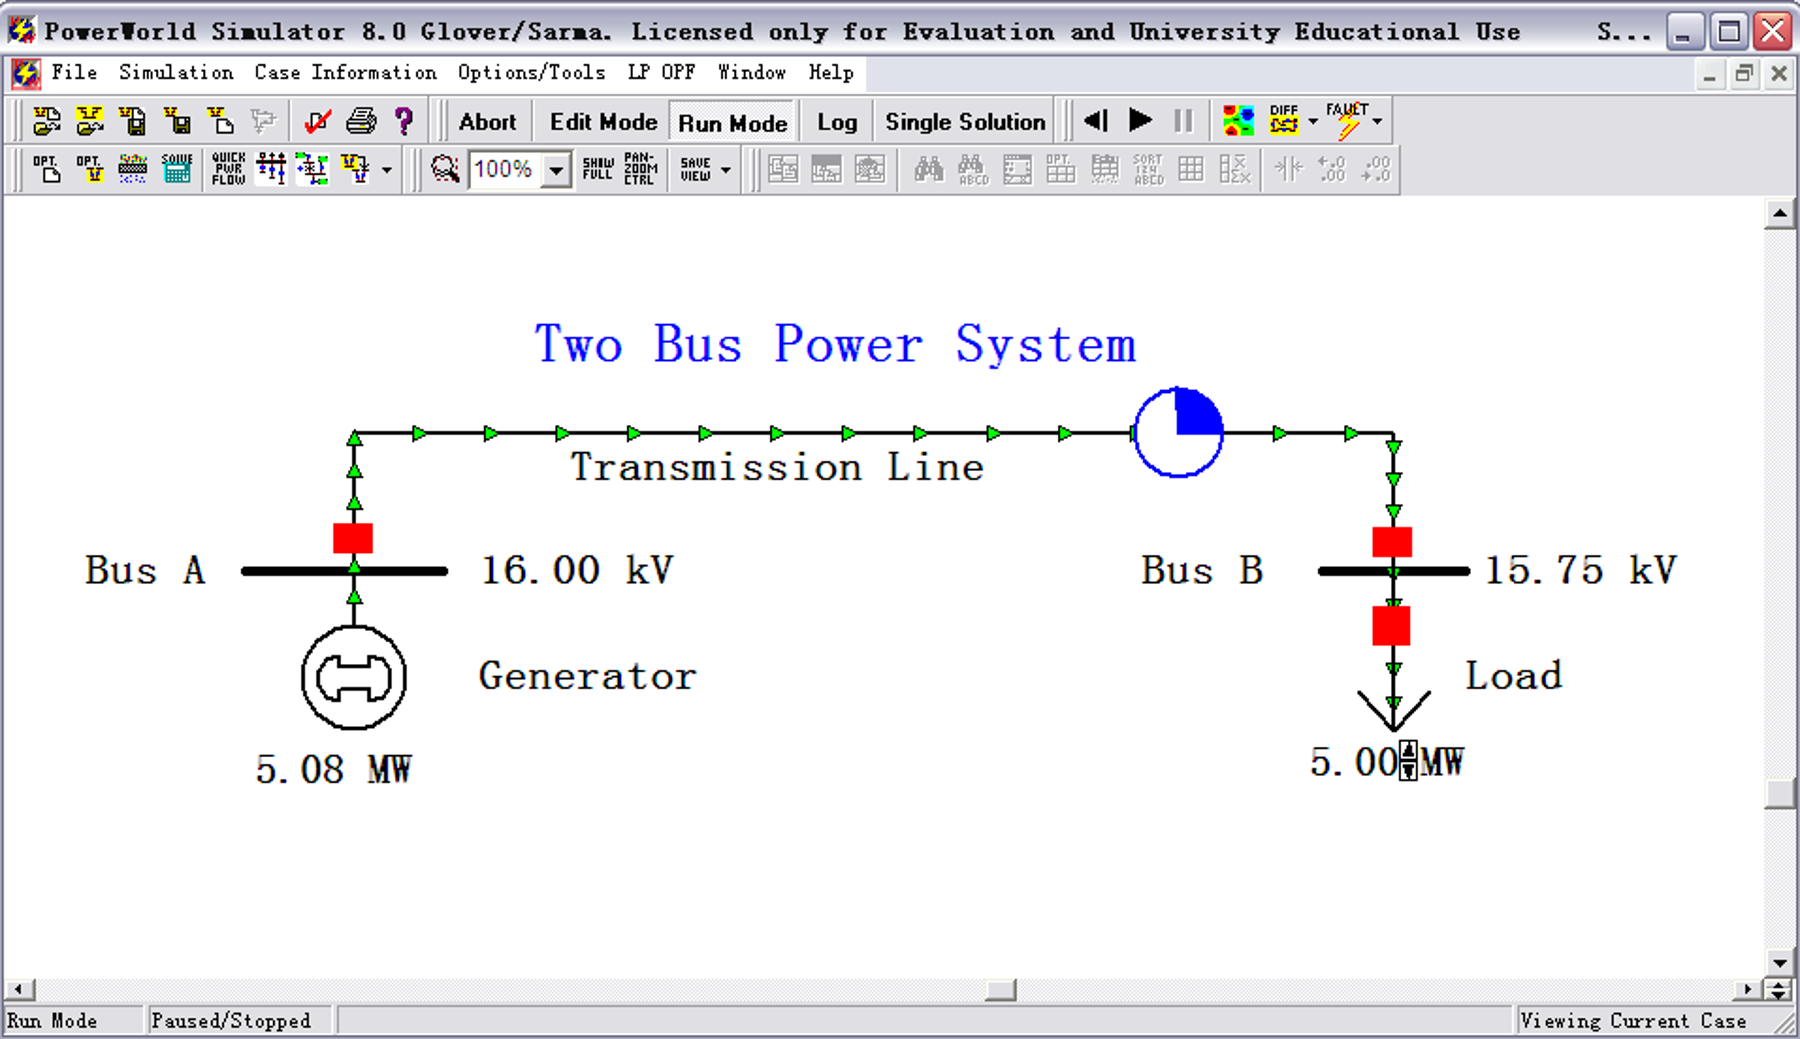
\includegraphics[width=\linewidth,height=.72\textheight,keepaspectratio]{assets/energy_assignment_p009_01.png}\caption{Diagram or recorded result: Seven-bus case data.}\label{fig:energy_assignment_p009_010}\end{figure}
\clearpage
\section{Part I: seven required experiments}

\begin{enumerate}

\item Build the case, select Run Mode, and solve with Gauss-Seidel one iteration at a time. Then clear Do Only One Iteration and allow up to 100 iterations. Inspect Bus Power Flows and Bus Real/\allowbreak{}Reactive Power Mismatches.

\item Repeat with Newton-Raphson and inspect the Jacobian through Case Information, Other, Power Flow Jacobian. Compare residual behavior under a common stopping rule.

\item Apply 0.95-1.05 per-unit voltage limits. Disconnect the bus-3 capacitor bank and record all voltage and loss changes.

\item Change the bus-1/\allowbreak{}bus-4 transformer tap to bring bus 3 toward 1.0 per unit while retaining all bus limits.

\item Add a parallel transformer between buses 1 and 4, first with identical parameters, then with twice the reactance. Examine sharing and voltage effects.

\item Remove line 3-4 and find how much bus-3 load must be shed to keep its voltage above 0.95 per unit.

\item Add an identical parallel line 3-4 and compare line flows and total losses.

\end{enumerate}
\begin{figure}[!htbp]\centering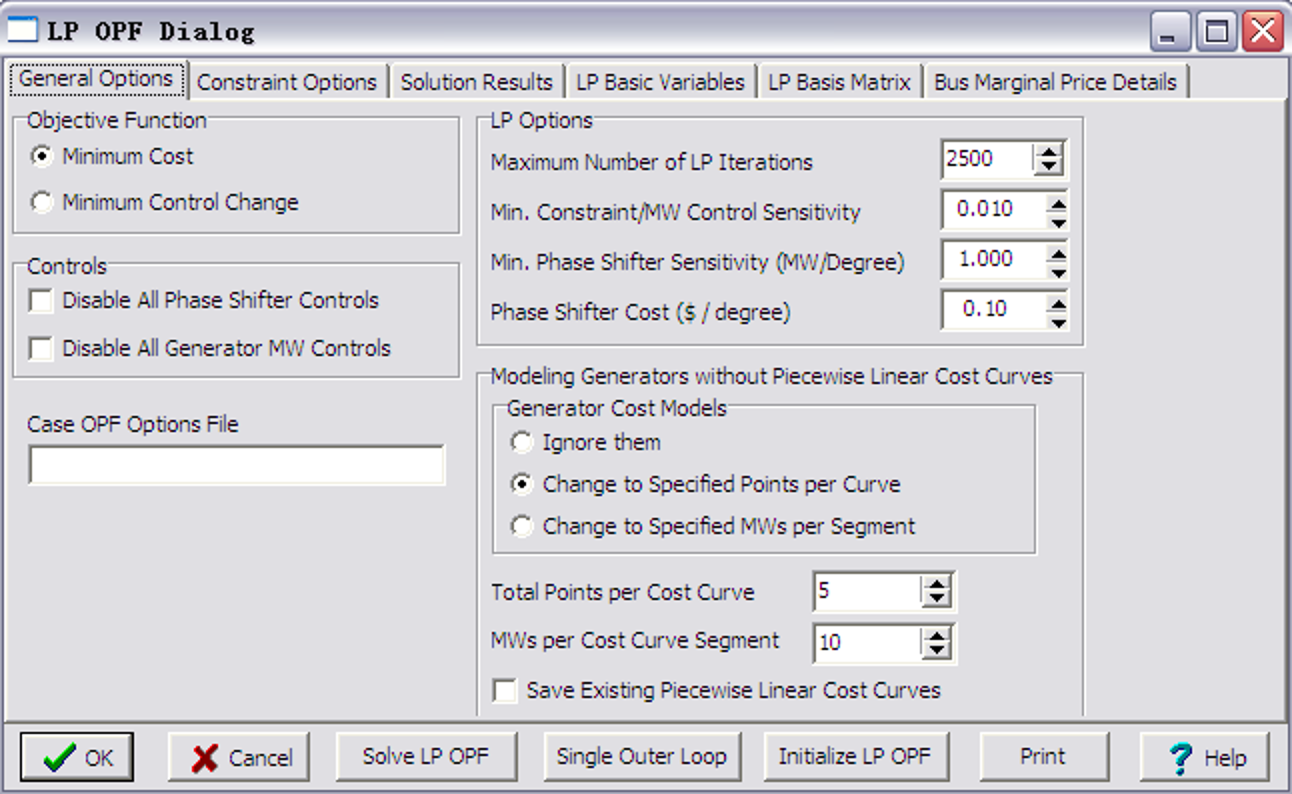
\includegraphics[width=\linewidth,height=.72\textheight,keepaspectratio]{assets/energy_assignment_p010_01.png}\caption{Diagram or recorded result: Part I: seven required experiments.}\label{fig:energy_assignment_p010_010}\end{figure}
\begin{figure}[!htbp]\centering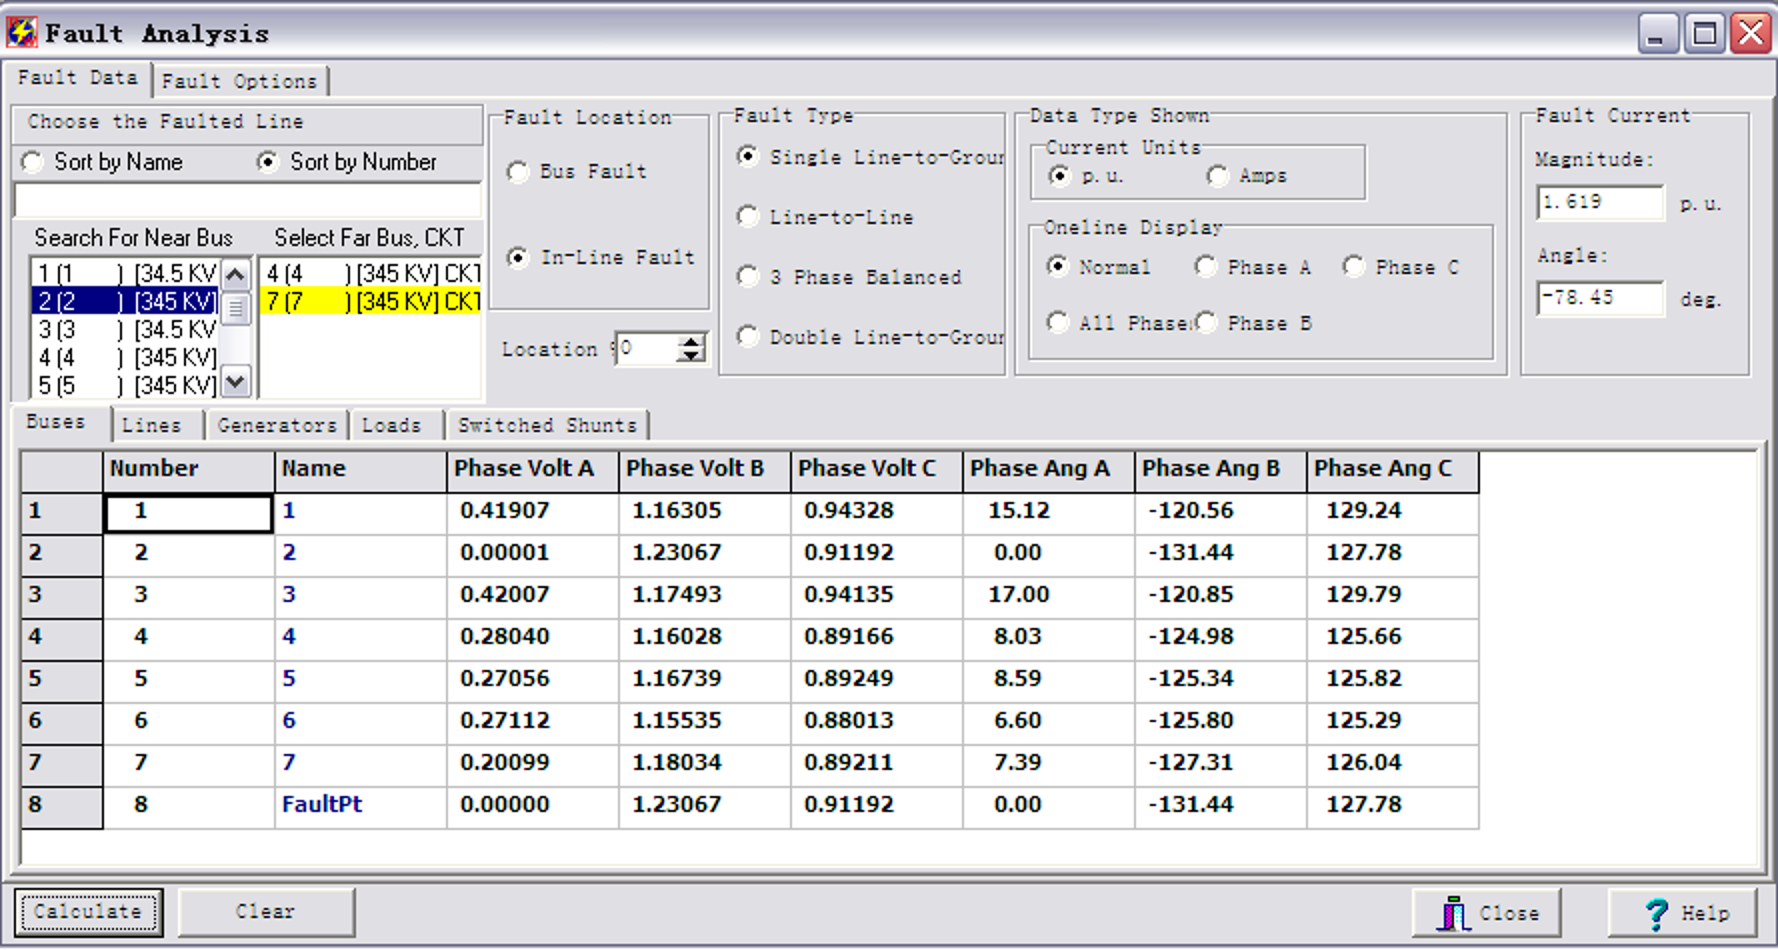
\includegraphics[width=\linewidth,height=.72\textheight,keepaspectratio]{assets/energy_assignment_p010_02.png}\caption{Diagram or recorded result: Part I: seven required experiments.}\label{fig:energy_assignment_p010_020}\end{figure}
\clearpage
\section{Part II and discussion}

Use the contingency-analysis tool with the stated +\allowbreak{}/\allowbreak{}-5-percent voltage criterion. Examine removal of line 3-4, removal of line 5-7, and replacing the bus-2 generator with a similar bus-3 generator. Record solve status, voltage/\allowbreak{}flow violations, and assumptions for each case. Discuss advantages of both solution methods;\allowbreak{} the role and limits of shunt compensation;\allowbreak{} topology, equipment, cost, and constraints needed for OPF;\allowbreak{} and ways to improve reliability/\allowbreak{}resilience. Distinguish proposed measures from verified contingency improvements. The original English Word assignment has been rendered to a 13-page PDF so that embedded equations, drawings, tables, and dialog figures remain readable.

\begingroup\small\setlength{\tabcolsep}{3pt}\renewcommand{\arraystretch}{1.18}\begin{longtable}{@{}p{0.1171\linewidth}p{0.1171\linewidth}p{0.1171\linewidth}p{0.1171\linewidth}p{0.1171\linewidth}p{0.1171\linewidth}p{0.1171\linewidth}@{}}
\caption{Part II and discussion - numerical data and parameters. (panel 1)}\label{tab:energy_assignment_p011_table10}\\\toprule
\textbf{Bus
No.} & \textbf{P
Generate
(MW)} & \textbf{Q
Generate
(MVar)} & \textbf{P
Loaded
(MW)} & \textbf{Q
Loaded
(MVar)} & \textbf{Bus
Type*} & \textbf{Q
Generate
Max.(MVar)} \\ \midrule\endfirsthead \textbf{Bus
No.} & \textbf{P
Generate
(MW)} & \textbf{Q
Generate
(MVar)} & \textbf{P
Loaded
(MW)} & \textbf{Q
Loaded
(MVar)} & \textbf{Bus
Type*} & \textbf{Q
Generate
Max.(MVar)} \\ \midrule\endhead
1 & 55.0 & 32.0 & 0.0 & 0.0 & 2 & 40.0 \\
2 & 82.0 & 33.0 & 26.0 & 0.0 & 1 & 40.0 \\
3 & 0.0 & 37.0 & 50.0 & 34.0 & 3 & 0.0 \\
4 & 0.0 & 0.0 & 0.0 & 0.0 & 3 & 0.0 \\
5 & 0.0 & 0.0 & 0.0 & 0.0 & 3 & 0.0 \\
6 & 0.0 & 0.0 & 40.0 & 23.0 & 3 & 0.0 \\
7 & 0.0 & 10.0 & 20.0 & 15.0 & 3 & 0.0 \\
\bottomrule\end{longtable}\endgroup
\begingroup\small\setlength{\tabcolsep}{3pt}\renewcommand{\arraystretch}{1.18}\begin{longtable}{@{}p{0.3000\linewidth}p{0.3000\linewidth}p{0.3000\linewidth}@{}}
\caption{Part II and discussion - numerical data and parameters. (panel 2)}\label{tab:energy_assignment_p011_table11}\\\toprule
\textbf{Bus
No.} & \textbf{Q
Generate
Min.(MVar)} & \textbf{Voltage
Level
(kV)} \\ \midrule\endfirsthead \textbf{Bus
No.} & \textbf{Q
Generate
Min.(MVar)} & \textbf{Voltage
Level
(kV)} \\ \midrule\endhead
1 & -6.0 & 34.5 \\
2 & -6.0 & 34.5 \\
3 & 0.0 & 345 \\
4 & 0.0 & 345 \\
5 & 0.0 & 345 \\
6 & 0.0 & 345 \\
7 & 0.0 & 345 \\
\bottomrule\end{longtable}\endgroup
\begin{figure}[!htbp]\centering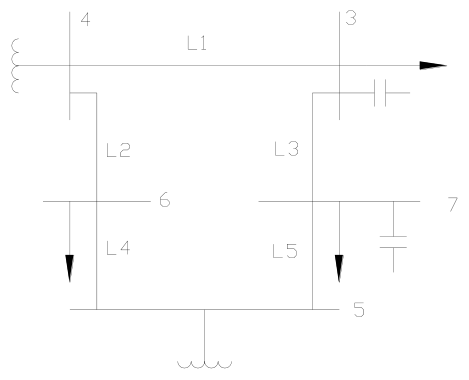
\includegraphics[width=\linewidth,height=.72\textheight,keepaspectratio]{assets/energy_assignment_p011_vector5.png}\caption{Diagram or recorded result: Part II and discussion.}\label{fig:energy_assignment_p011_vector50}\end{figure}
\begin{figure}[!htbp]\centering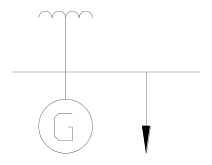
\includegraphics[width=\linewidth,height=.72\textheight,keepaspectratio]{assets/energy_assignment_p011_vector7.png}\caption{Diagram or recorded result: Part II and discussion.}\label{fig:energy_assignment_p011_vector70}\end{figure}
\clearpage
\end{document}